\chap{复平面}
\section{介绍}
一些学科的历史往往是令人兴奋的读物,尤其是在对日期或先有技术存在争议的情况下。澄清谁在别人之前做了某事是历史学家的工作,他们可以帮助揭示谁应该为某一事件负责,谁应该居功至伟。要从日记、书籍和私人信件中理清事件的来龙去脉,并将它们按时间顺序排列在一起,需要具备学科知识、坚韧的毅力和客观的分析。

对于大多数研究学科来说,有两个日期对于确定优先权非常重要:论文提交发表的日期和被接受的论文发表的日期。这样的协议似乎是一个公平的方案,但前提是要有一个高效的邮政系统、一个公正的同行评审系统,以及其他许多条件。

在数学和科学领域,一些研究人员并不总是有信心将一个萌芽的想法发表出来,如果不发表,这个想法要么留在他们的脑海里,要么放在他们桌上的笔记本里,在研究人员死后可能被发现,也可能不被发现。对研究人员来说,不幸的是,人的脑袋并不是历史学家方便的信息存放处!

有时,数学论文会出现在与其他学科相关的期刊上,可以理解的是,这些期刊并不一定受到数学界的监督。同样,历史学家或好奇的学者通过巧妙的侦查工作,也会将复杂的优先权、归属问题浮出水面,在某些情况下,还会引起令人不快的剽窃嫌疑。

复数平面的发明是一个完美的例子,它说明了当数学思想的官方发布渠道被 "双关 "时,发明者会遇到怎样的严重问题。让我们看看发生了什么。

\section{一些历史}
一切始于 1813 年,瑞士业余数学家让-罗伯特-阿尔冈(Jean-Robert Argand,1768-1822 年)在他私人资助的一本 "小册子 "中发表了他关于复数几何解释的想法:关于几何构造中虚量表示方法的论文(Essai sur une manière de représenter les quantités imaginaires dans les constructions géométriques)\cite{bib4-1}。

这本小册子并没有广泛传播,更糟糕的是,它并没有 Argand 的名字!1813 年,Jacques Français 在一篇论文中重新发表了复平面的想法,并要求最初想法的匿名作者透露自己的身份。Argand 站了出来,他的发明得到了认可,如今复平面被称为 Argand 图。1874 年,Gauthier-Villars 出版社出版了 Argand 著作的第二版\cite{bib4-2}。

Unbeknown to Argand-and everyone else at the time-a Norwegian surveyor Caspar Wessel (1745-1818), had been triangulating Denmark and developing mathematical techniques to simplify his work. One of these ideas was the original idea of adding vectorial quantities, the other was the geometric interpretation of complex numbers.

Wessel presented his first and only mathematical paper describing his complex plane to a meeting of the Royal Danish Academy in 1797, and it was published in the Academy's Mémoires in 1799. Wessel's paper remained hidden from the mathematical community for almost a century, when it was discovered in 1895 by the Danish mathematician Sophus Christian Juel (1855-1935). However, although everyone now agrees that Wessel was the first person to invent the complex plane, it still bears Argand's name.

But it doesn't end there! The Scottish mathematician Peter Guthrie Tait (18311901), wrote in his book An Elementary Treatise on Quaternions:

Wallis, in the end of the seventeenth century, proposed to represent the impossible roots, of a quadratic equation by going out of the line on which, if real they would have been laid off. His construction is equivalent to the consideration of $\sqrt{-1}$ as a directed unit line perpendicular to that on which real quantities are measured. [3]

John Wallis (1616-1703), was a gifted English mathematician [4], and it is believed that Argand, Warren, and others, extended the results of Wallis and De Moivre, who had done some early work on the complex plane.

\section{复平面}
One of the people associated with the development of complex numbers was the brilliant Swiss mathematician Leonhard Euler (1707-1783). Euler proved the identity:

$$
    e^{i \theta}=\cos \theta+i \sin \theta
$$

and when $\theta=\pi$, one of the most beautiful formulae in mathematics emerges:

$$
    e^{i \pi}=-1
$$

or

$$
    e^{i \pi}+1=0
$$

which integrates five important constants: $0,1, e, \pi$ and $i$, as well as the basic arithmetic operations: addition, multiplication and exponentiation.

Another consequence of this formula arises when $\theta=\pi / 2$ :

$$
    e^{i \pi / 2}=\cos \left(\frac{\pi}{2}\right)+i \sin \left(\frac{\pi}{2}\right)=i
$$

therefore,

$$
    \begin{aligned}
        i^{i} & =\left(e^{i \pi / 2}\right)^{i} \\
              & =e^{i^{2} \pi / 2}              \\
              & =e^{-\pi / 2}                   \\
              & \approx 0.207879576 .
    \end{aligned}
$$

which shows that the imaginary unit raised to itself equals a real number!

In Chap. 3 we saw that the powers of imaginary $i$ give rise to two sequences $(1, i,-1,-i, 1, \ldots)$ and $(1,-i,-1, i, 1, \ldots)$ which bear a striking resemblance to the patterns $(x, y,-x,-y, x, \ldots)$ and $(x,-y,-x, y, x, \ldots)$ that arise when rotating about the Cartesian axes in an counter-clockwise and clockwise direction, respectively. This resemblance is no coincidence, as complex numbers belong to a two-dimensional plane called the complex plane, which we will now describe.

The complex plane enables us to visualise complex numbers using the horizontal axis to record the real part, and the vertical axis to record the imaginary part, as shown in Fig. 4.1.

The figure also shows a circle with unit radius passing through the points $1, i,-1,-i$, which is the sequence associated with increasing powers of $i$. We can see the positions for $i^{0}=1, i^{1}=i, i^{2}=-1, i^{3}=-i$ and $i^{4}=1$, which suggest that multiplying by $i$ is equivalent to rotating through $90^{\circ}$.

To demonstrate this rotational effect, Fig. 4.2 shows the complex plane with four complex numbers:

$$
    p=2+i, \quad q=-1+2 i, \quad r=-2-i, \quad s=1-2 i
$$

which are $90^{\circ}$ apart. Fig. 4.1 The complex plane with the unit circle

Fig. 4.2 The complex plane with four complex numbers
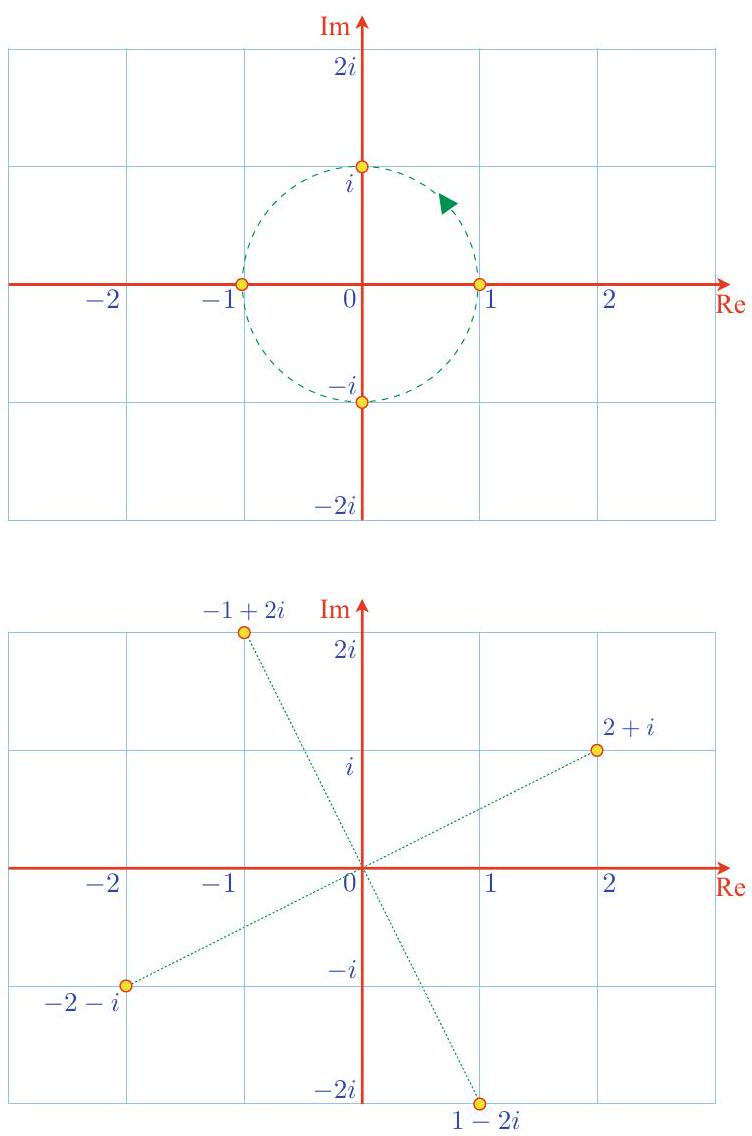
\includegraphics[max width=\textwidth, center]{2023_04_20_41f1ceac5a31dc7d1b59g-069}

The point $p$ is rotated $90^{\circ}$ to $q$ by multiplying it by $i$ :

$$
    \begin{aligned}
        i(2+i) & =2 i+i^{2} \\
               & =-1+2 i .
    \end{aligned}
$$

The point $q$ is rotated another $90^{\circ}$ to $r$ by multiplying it by $i$ :

$$
    \begin{aligned}
        i(-1+2 i) & =-i+2 i^{2} \\
                  & =-2-i
    \end{aligned}
$$

The point $r$ is rotated another $90^{\circ}$ to $s$ by multiplying it by $i$ :

$$
    \begin{aligned}
        i(-2-i) & =-2 i-i^{2} \\
                & =1-2 i
    \end{aligned}
$$

Finally, the point $s$ is rotated $90^{\circ}$ back to $p$ by multiplying it by $i$ :

$$
    \begin{aligned}
        i(1-2 i) & =i-2 i^{2} \\
                 & =2+i
    \end{aligned}
$$

We also discovered in Chap. 3 that the sequence associated with increasing negative powers: $(1,-i,-1, i, \ldots)$ is a rotation in a clockwise direction, and implies that dividing a complex number by $i$ rotates it $90^{\circ}$ clockwise. However, we showed that $i^{-1}=-i$, and it is much easier to multiply a complex number by $-i$ than divide it by $i$. So let's repeat the above exercise to prove this point.

The point $p$ is rotated $-90^{\circ}$ to $s$ by multiplying it by $-i$ :

$$
    \begin{aligned}
        -i(2+i) & =-2 i-i^{2} \\
                & =1-2 i
    \end{aligned}
$$

The point $s$ is rotated another $-90^{\circ}$ to $r$ by multiplying it by $-i$ :

$$
    \begin{aligned}
        -i(1-2 i) & =-i+2 i^{2} \\
                  & =-2-i .
    \end{aligned}
$$

The point $r$ is rotated another $90^{\circ}$ to $q$ by multiplying it by $-i$ :

$$
    \begin{aligned}
        -i(-2-i) & =2 i+i^{2} \\
                 & =-1+2 i .
    \end{aligned}
$$

Finally, the point $q$ is rotated $90^{\circ}$ back to $p$ by multiplying it by $-i$ :

$$
    \begin{aligned}
        -i(-1+2 i) & =i-2 i^{2} \\
                   & =2+i
    \end{aligned}
$$

Thus a complex number is rotated $\pm 90^{\circ}$ by multiplying it by $\pm i$.

In Chap. 3 we saw that the roots of $\sqrt{ \pm i}$ are

$$
    \begin{aligned}
         & \sqrt{+i}= \pm \frac{\sqrt{2}}{2}(1+i) \\
         & \sqrt{-i}= \pm \frac{\sqrt{2}}{2}(1-i)
    \end{aligned}
$$

and are shown in Fig. 4.3. Note that the individual roots are $180^{\circ}$ apart, which suggests that angles have something to do with their action. For example, the positive root of $\sqrt{i}$ is $\sqrt{2} / 2(1+i)$ and is $45^{\circ}$ from the real axis. Multiplying this root by itself rotates it $45^{\circ}$ to the $i$ axis. Similarly, the negative root is $-\sqrt{2} / 2(1+i)$ and is $225^{\circ}$ from the real axis. Multiplying this root by itself rotates it $225^{\circ}$ to the $i$ axis. The same is true for the roots of $\sqrt{-i}$. Fig. 4.3 The complex roots of $\sqrt{ \pm i}$

\begin{center}
    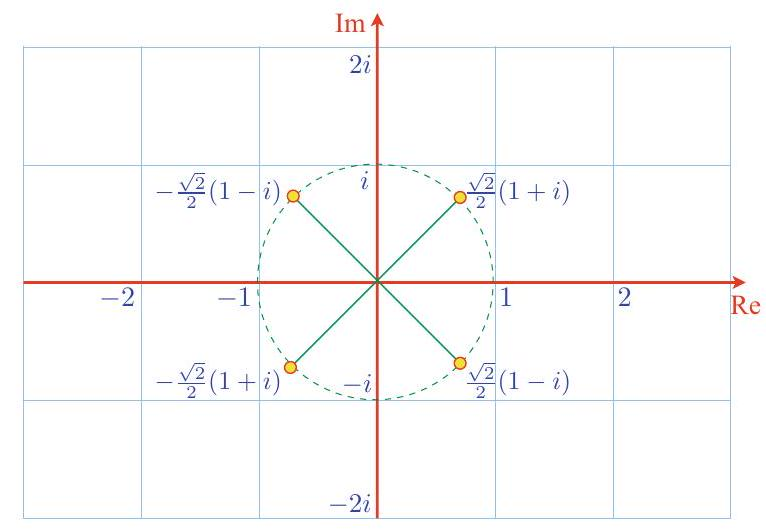
\includegraphics[max width=\textwidth]{2023_04_20_41f1ceac5a31dc7d1b59g-071}
\end{center}

These observations seem to suggest that we can construct a complex number capable of rotating another complex number through any angle. Which is true and is covered next.

\section{极坐标表示法}
Placing a complex number on the complex plane leads us to polar representation where we form a line from the origin to the complex number as shown in Fig. 4.4. The length of the line is $r$ and equals $\sqrt{a^{2}+b^{2}}$, which is why the norm of a complex number is defined using the Pythagorean formula:

$$
    r=|z|=\sqrt{a^{2}+b^{2}}
$$

The angle $\theta$ between the line and the real axis is called the argument of $z$ and written:

$$
    \arg (z)=\theta
$$

where,

$$
    \tan \theta=\frac{b}{a}
$$

1st quadrant: $a>0, b>0$,

$\theta=\arctan \left(\frac{b}{a}\right)$

2nd \& 3rd quadrant: $a<0$,

$$
    \theta=\arctan \left(\frac{b}{a}\right)+\pi
$$

4th quadrant: $a>0, b<0$,

$$
    \theta=\arctan \left(\frac{b}{a}\right)+2 \pi
$$

Fig. 4.4 Polar

representation of a complex number

\begin{center}
    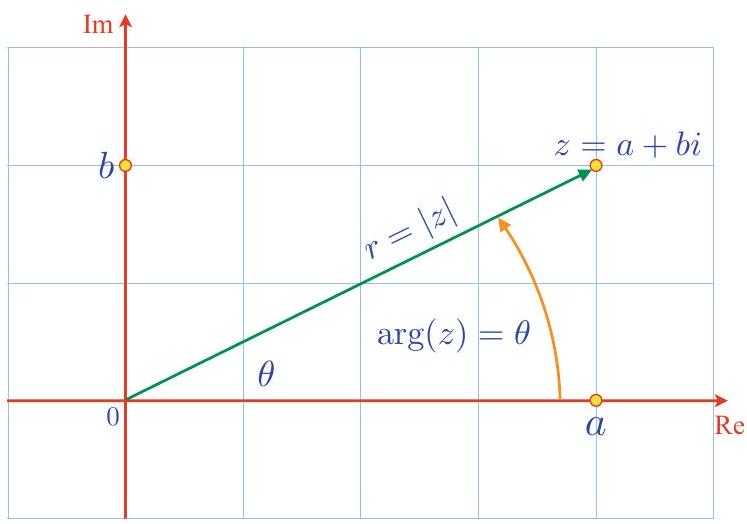
\includegraphics[max width=\textwidth]{2023_04_20_41f1ceac5a31dc7d1b59g-072}
\end{center}

We can see from Fig. 4.4 that the horizontal component of $z$ is $r \cos \theta$ and the vertical component is $r \sin \theta$, which permits us to write

$$
    \begin{aligned}
        z & =a+b i                          \\
          & =r \cos \theta+r i \sin \theta  \\
          & =r(\cos \theta+i \sin \theta) .
    \end{aligned}
$$

As mentioned above, one of Euler's discoveries is the identity relating the power series for $e^{\theta}, \sin \theta$ and $\cos \theta$ :

$$
    e^{i \theta}=\cos \theta+i \sin \theta
$$

which permits us to write

$$
    z=r e^{i \theta}
$$

Armed with this discovery, we are now in a position to revisit the product and quotient of two complex numbers using polar representation. For example, given the following complex numbers:

$$
    \begin{aligned}
        z & =r e^{i \theta} \\
        w & =s e^{i \phi}
    \end{aligned}
$$

their product is

$$
    \begin{aligned}
        z w & =r s e^{i \theta} e^{i \phi}                  \\
            & =r s e^{i(\theta+\phi)}                       \\
            & =r s[\cos (\theta+\phi)+i \sin (\theta+\phi)]
    \end{aligned}
$$

So the product of two complex numbers creates a third one with norm

$$
    |z w|=r s
$$

and argument

$$
    \arg (z w)=\theta+\phi
$$

where the angles are added.

Next, the quotient:

$$
    \begin{aligned}
        \frac{z}{w} & =\frac{r e^{i \theta}}{s e^{i \phi}}                  \\
                    & =\frac{r}{s} e^{i(\theta-\phi)}                       \\
                    & =\frac{r}{s}[\cos (\theta-\phi)+i \sin (\theta-\phi)]
    \end{aligned}
$$

where the norm is

$$
    \left|\frac{z}{w}\right|=\frac{r}{s}
$$

and the argument is

$$
    \arg \left(\frac{z}{w}\right)=\theta-\phi
$$

where the angles are subtracted.

Let's employ these formulae with an example. Figure 4.5 shows two complex numbers:

$$
    \begin{gathered}
        z=2+2 i \\
        w=-1+i
    \end{gathered}
$$

which in polar form are

$$
    \begin{aligned}
        z & =2 \sqrt{2}\left(\cos 45^{\circ}+i \sin 45^{\circ}\right)=2 \sqrt{2} e^{i \pi / 4}   \\
        w & =\sqrt{2}\left(\cos 135^{\circ}+i \sin 135^{\circ}\right)=\sqrt{2} e^{i 3 \pi / 4} .
    \end{aligned}
$$

Using normal complex algebra, the product $z w$ is

$$
    z w=(2+2 i)(-1+i)=-4
$$

and using polar form: Fig. 4.5 The product and quotient of two complex numbers

\begin{center}
    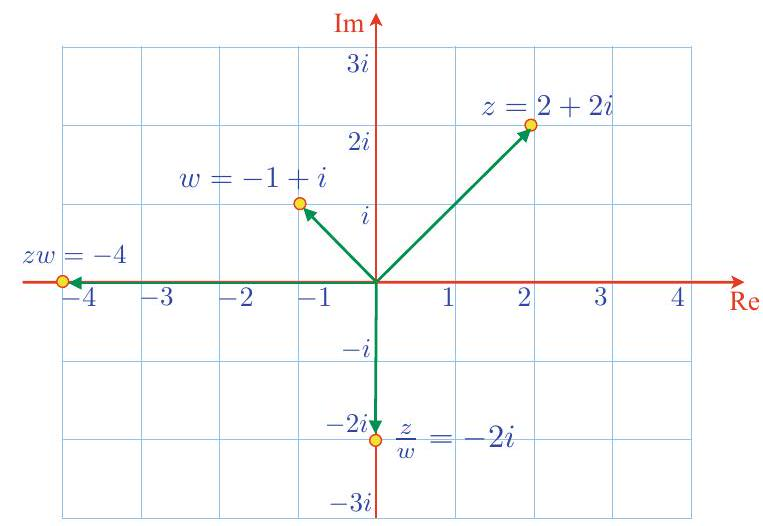
\includegraphics[max width=\textwidth]{2023_04_20_41f1ceac5a31dc7d1b59g-074}
\end{center}

$$
    \begin{aligned}
        |z w|      & =2 \sqrt{2} \sqrt{2}=4              \\
        \arg (z w) & =45^{\circ}+135^{\circ}=180^{\circ}
    \end{aligned}
$$

which encode -4 .

Now let's compute the quotient $z / w$ using normal complex algebra, then the polar form.

$$
    \begin{aligned}
        \frac{z}{w} & =\frac{(2+2 i)}{(-1+i)} \frac{(-1-i)}{(-1-i)} \\
                    & =\frac{-2-2 i-2 i-2 i^{2}}{1+1}               \\
                    & =-2 i .
    \end{aligned}
$$

Next, using polar form:

$$
    \begin{aligned}
        \left|\frac{z}{w}\right|      & =\frac{2 \sqrt{2}}{\sqrt{2}}=2      \\
        \arg \left(\frac{z}{w}\right) & =45^{\circ}-135^{\circ}=-90^{\circ}
    \end{aligned}
$$

which encode the complex number $-2 i$. These results are shown in Fig. 4.5.

We can also use Euler's formula to compute $\sqrt{i}$ as follows:

$$
    e^{i \theta}=\cos \theta+i \sin \theta
$$

substituting $\theta=\pi / 2$ we have

$$
    e^{i \pi / 2}=\cos \left(\frac{\pi}{2}\right)+i \sin \left(\frac{\pi}{2}\right)=i
$$

taking the square root of both sides, we have

$$
    \begin{aligned}
        \pm e^{i \pi / 4}                                                                 & =\sqrt{i} \\
        \pm\left[\cos \left(\frac{\pi}{4}\right)+i \sin \left(\frac{\pi}{4}\right)\right] & =\sqrt{i} \\
        \pm \frac{\sqrt{2}}{2}(1+i)                                                       & =\sqrt{i}
    \end{aligned}
$$

To find $\sqrt{-i}$ we substitute $\theta=-\pi / 2$ :

$$
    \begin{aligned}
        e^{-i \pi / 2} & =\cos \left(-\frac{\pi}{2}\right)+i \sin \left(-\frac{\pi}{2}\right)=-i \\
                       & =\cos \left(\frac{\pi}{2}\right)-i \sin \left(\frac{\pi}{2}\right)=-i
    \end{aligned}
$$

taking the square root of both sides, we have

$$
    \begin{aligned}
        \pm e^{-i \pi / 4}                                                                & =\sqrt{-i} \\
        \pm\left[\cos \left(\frac{\pi}{4}\right)-i \sin \left(\frac{\pi}{4}\right)\right] & =\sqrt{-i} \\
        \pm \frac{\sqrt{2}}{2}(1-i)                                                       & =\sqrt{-i}
    \end{aligned}
$$

Higher roots can be found using a similar technique.

\section{转子}
The polar form brings home the fact that multiplying $z=r e^{i \theta}$ with norm $r$, by $w=s e^{i \phi}$ with norm $s$, creates a third complex number with norm $r s$. Therefore, to avoid scaling $z, w$ must have a norm of unity. Under such conditions, $w$ acts as a rotor. For example, multiplying $4+5 i$ by $1+0 i$ leaves it unscaled and unrotated. However, multiplying $4+5 i$ by $0+i$ rotates it by $90^{\circ}$ without any scaling.

Therefore, to rotate $2+2 i$ by $45^{\circ}$, we must multiply it by $e^{i \pi / 4}$ :

$$
    \begin{aligned}
        e^{i \pi / 4}                  & =\cos 45^{\circ}+i \sin 45^{\circ}=\frac{\sqrt{2}}{2}(1+i) \\
        \frac{\sqrt{2}}{2}(1+i)(2+2 i) & =\frac{\sqrt{2}}{2} 4 i                                    \\
                                       & =2 \sqrt{2} i
    \end{aligned}
$$

So $e^{i \theta}$ rotates any complex number through an angle $\theta$.

To rotate a complex number $x+y i$ through an angle $\theta$ we can multiply it by the rotor $\cos \theta+i \sin \theta$

$$
    \begin{aligned}
        x^{\prime}+y^{\prime} i & =(\cos \theta+i \sin \theta)(x+y i)                         \\
                                & =x \cos \theta-y \sin \theta+i(x \sin \theta+y \cos \theta)
    \end{aligned}
$$

which in matrix form is:

$$
    \left[\begin{array}{r}
            x^{\prime} \\
            i y^{\prime}
        \end{array}\right]=\left[\begin{array}{rr}
            \cos \theta & -\sin \theta \\
            \sin \theta & \cos \theta
        \end{array}\right]\left[\begin{array}{c}
            x \\
            i y
        \end{array}\right]
$$

Before moving on let's consider the effect the complex conjugate of a rotor has on rotational direction, and we can do this by multiplying $x+y i$ by the rotor $\cos \theta-$ $i \sin \theta$ :

$$
    \begin{aligned}
        x^{\prime}+y^{\prime} i & =(\cos \theta-i \sin \theta)(x+y i)                          \\
                                & =x \cos \theta+y \sin \theta+i(-x \sin \theta+y \cos \theta)
    \end{aligned}
$$

and in matrix form is

$$
    \left[\begin{array}{r}
            x^{\prime} \\
            i y^{\prime}
        \end{array}\right]=\left[\begin{array}{rr}
            \cos \theta  & \sin \theta \\
            -\sin \theta & \cos \theta
        \end{array}\right]\left[\begin{array}{c}
            x \\
            i y
        \end{array}\right]
$$

which is a rotation of $-\theta$ about the origin.

Therefore, we define a rotor $\mathbf{R}_{\theta}$ and its conjugate $\mathbf{R}_{\theta}^{\dagger}$ as

$$
    \begin{aligned}
         & \mathbf{R}_{\theta}=\cos \theta+i \sin \theta           \\
         & \mathbf{R}_{\theta}^{\dagger}=\cos \theta-i \sin \theta
    \end{aligned}
$$

where $\mathbf{R}_{\theta}$ rotates $+\theta$, and $\mathbf{R}_{\theta}^{\dagger}$ rotates $-\theta$. Note the use of the dagger $\dagger$ symbol.

\section{总结}
在这一章中,我们发现了利用复平面对复数的图形化解释。欧拉公式 $e^{i \theta}=\cos \theta+i \sin \theta$ 允许我们将复数表示为$e$的虚次幂,从而使我们可以轻松地计算乘积和商。总之,这些想法让我们产生了转子的想法,而转子将使用四元数来开发。

\subsection{定义总结}
\begin{tcolorbox}[breakable, enhanced,title = {复数}]
    $$
        \begin{aligned}
            z   & =a+b i              \\
            |z| & =\sqrt{a^{2}+b^{2}}
        \end{aligned}
    $$
\end{tcolorbox}

\begin{tcolorbox}[breakable, enhanced,title = {极坐标形式}]
    $$
        \begin{aligned}
            z           & =r e^{i \theta}               \\
            z           & =r(\cos \theta+i \sin \theta) \\
            r           & =|z|                          \\
            \tan \theta & =b / a                        \\
            \theta      & =\arg (z) .
        \end{aligned}
    $$

    $$
        \begin{aligned}
            \text{第一象限:   }     & a>0, b>0  &  & \theta=\arctan \left(\frac{b}{a}\right).       \\
            \text{第二、第三象限: } & a<0,      &  & \theta=\arctan \left(\frac{b}{a}\right)+\pi.   \\
            \text{第四象限:  }      & a>0, b<0, &  & \theta=\arctan \left(\frac{b}{a}\right)+2 \pi.
        \end{aligned}
    $$
\end{tcolorbox}

\begin{tcolorbox}[breakable, enhanced,title = {乘积}]
    $$
        \begin{aligned}
            z   & =r e^{i \theta}                                 \\
            w   & =s e^{i \phi}                                   \\
            z w & =r s e^{i(\theta+\phi)}                         \\
                & =r s[\cos (\theta+\phi)+i \sin (\theta+\phi)] .
        \end{aligned}
    $$
\end{tcolorbox}
\begin{tcolorbox}[breakable, enhanced,title = {商}]
    $$
        \begin{aligned}
            \frac{z}{w} & =\frac{r}{s} e^{i(\theta-\phi)}                         \\
                        & =\frac{r}{s}[\cos (\theta-\phi)+i \sin (\theta-\phi)] .
        \end{aligned}
    $$
\end{tcolorbox}

\begin{tcolorbox}[breakable, enhanced,title = {转子}]
    $$
        \begin{aligned}
             & \mathbf{R}_{\theta}=\cos \theta+i \sin \theta             \\
             & \mathbf{R}_{\theta}^{\dagger}=\cos \theta-i \sin \theta .
        \end{aligned}
    $$
\end{tcolorbox}



\section{样例}
下面是一些进一步运用上述思想的例子。在某些情况下,需要进行测试以确认结果。

\begin{myexample}{用 \boldmath $i$ 旋转复数}{theoexample}
从 $1+2 i$ 开始,将得到的复数乘以 $i$四次,并在复数平面上绘出结果。

将点 $p$ 旋转 $90^{\circ}$ 至 $q$ 是通过乘以 $i$,:
$$
    \begin{aligned}
        i(1+2 i) & =i+2 i^{2} \\
                 & =-2+i .
    \end{aligned}
$$
通过乘以 $i$,点 $q$ 又旋转了 $90^{\circ}$ 至 $r$ :
$$
    \begin{aligned}
        i(-2+i) & =-2 i+i^{2} \\
                & =-1-2 i .
    \end{aligned}
$$

通过乘以 $i$,点 $r$ 又旋转了 $90^{\circ}$ 至 $s$:
$$
    \begin{aligned}
        i(-1-2 i) & =-i-2 i^{2} \\
                  & =2-i .
    \end{aligned}
$$

最后,通过乘以 $i$,将点 $s$ 旋转 $90^{\circ}$ 回到 $p$:
$$
    \begin{aligned}
        i(2-i) & =2 i-i^{2} \\
               & =2+i .
    \end{aligned}
$$

图\ref{fig:4.6} 显示了由 $90^{\circ}$ 分隔的四个复数。
\end{myexample}

\begin{figure}[htbp]
    \centering
    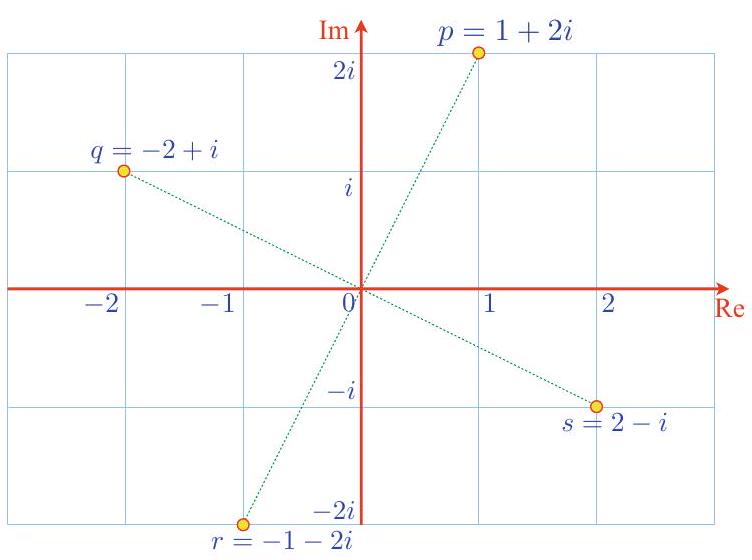
\includegraphics[max width=0.8\textwidth]{2023_04_20_41f1ceac5a31dc7d1b59g-078}
    \caption{有四个复数的复平面}
    \label{fig:4.6}
\end{figure}

\begin{myexample}{使用极坐标形式计算积和商}{theoexample}
用极坐标形式计算积 $z w$ 和商 $z / w$。
$$
    \begin{gathered}
        z=3+3 i \\
        w=-1-i .
    \end{gathered}
$$
乘积:
$$
    \begin{aligned}
        z          & =3 \sqrt{2}\left(\cos 45^{\circ}+i \sin 45^{\circ}\right)=3 \sqrt{2} e^{i \pi / 4} \\
        w          & =\sqrt{2}\left(\cos 225^{\circ}+i \sin 225^{\circ}\right)=\sqrt{2} e^{i 5 \pi / 4} \\
        |z w|      & =3 \sqrt{2} \sqrt{2}=6                                                             \\
        \arg (z w) & =45^{\circ}+225^{\circ}=270^{\circ}
    \end{aligned}
$$

编码复数 $-6 i$。

测试: 使用普通复数代数,乘积 $z w$ 是
$$
    z w=(3+3 i)(-1-i)=-6 i
$$

商:
$$
    \begin{aligned}
        |z|                           & =3 \sqrt{2}                         \\
        |w|                           & =\sqrt{2}                           \\
        \left|\frac{z}{w}\right|      & =3 \sqrt{2} / \sqrt{2}=3            \\
        \arg \left(\frac{z}{w}\right) & =45^{\circ}-225^{\circ}=180^{\circ}
    \end{aligned}
$$

编码复数 -3 。

测试: 使用普通复代数,商 $z / w$ 是
$$
    \begin{aligned}
        \frac{z}{w} & =\frac{(3+3 i)}{(-1-i)} \frac{(-1+i)}{(-1+i)} \\
                    & =\frac{-6}{2}                                 \\
                    & =-3
    \end{aligned}
$$
并与极坐标形式一致。
\end{myexample}


\begin{myexample}{设计一个旋转复数$30^{\circ}$的转子 }{theoexample}
设计一个转子,使复数在不缩放的情况下旋转 $30^{\circ}$ 。首先
$$
    e^{i \theta}=\cos \theta+i \sin \theta
$$

令 $\theta=30^{\circ}=\pi / 6$

$$
    \begin{aligned}
        e^{i \pi / 6} & =\cos 30^{\circ}+i \sin 30^{\circ} \\
                      & =\frac{\sqrt{3}}{2}+\frac{1}{2} i  \\
                      & =\frac{1}{2}(\sqrt{3}+i) .
    \end{aligned}
$$

测试: 让我们用这个转子将 $1+0 i$ 旋转三次,直到 $i$。
$$
    \begin{aligned}
        \frac{1}{2}(\sqrt{3}+i) \frac{1}{2}(\sqrt{3}+i) \frac{1}{2}(\sqrt{3}+i) 1 & =\frac{1}{8}(\sqrt{3}+i)(\sqrt{3}+i)(\sqrt{3}+i) \\
                                                                                  & =\frac{1}{8}(2+2 \sqrt{3} i)(\sqrt{3}+i)         \\
                                                                                  & =\frac{1}{8}(2 \sqrt{3}-2 \sqrt{3}+2 i+6 i)      \\
                                                                                  & =i
    \end{aligned}
$$
\end{myexample}

\begin{myexample}{设计一个将复数旋转 $-60^{\circ}$ 的转子}{theoexample}
设计一个转子,使复数在不缩放的情况下旋转$-60^{\circ}$。首先
$$
    e^{i \theta}=\cos \theta+i \sin \theta
$$

令 $\theta=-60^{\circ}=-\pi / 3$
$$
    \begin{aligned}
        e^{-i \pi / 3} & =\cos \left(-60^{\circ}\right)+i \sin \left(-60^{\circ}\right) \\
                       & =\frac{1}{2}-\frac{\sqrt{3}}{2} i                              \\
                       & =\frac{1}{2}(1-\sqrt{3} i)
    \end{aligned}
$$
\end{myexample}









\begin{thebibliography}{99}
    \bibitem{bib4-1} Argand, J.R.: \href{http://www-history.mcs.st-andrews.ac.uk/Mathematicians/Argand.html}{http://www-history.mcs.st-andrews.ac.uk/Mathematicians/Argand.html}
    \bibitem{bib4-2} Argand, J.R.: Essai sur une manière de représenter les quantités imaginaires dans les constructions géométriques, 2nd edn. Gauthier-Villars, Paris (1874)
    \bibitem{bib4-3} Tait, P.G.: Elementary Treatise on Quaternions. Cambridge University Press, Cambridge (1867)
    \bibitem{bib4-4} Wallis, J.: \href{http://www-history.mcs.st-andrews.ac.uk/Mathematicians/Wallis.html}{http://www-history.mcs.st-andrews.ac.uk/Mathematicians/Wallis.html}
\end{thebibliography}
